


%请使用xelatex编译
\documentclass[11pt,addpoints,answers]{exam}


% required macros -- get header.tex file from course web page
% !Mode:: "TeX:UTF-8"
% !TEX root=./hw1.tex
\usepackage{xeCJK}    % 写中文要用到
\usepackage{tikz}
\usepackage{amsmath,amsfonts,amssymb,amsthm}
\usepackage{fullpage}
\usepackage{times}
\usepackage{hyperref}
\usepackage{pdfsync}
\usepackage{microtype}
\usepackage{color}
\usepackage{cleveref}
\crefformat{footnote}{#2\footnotemark[#1]#3}
\definecolor{light-gray}{gray}{0.5}

\renewcommand{\tablename}{表}
\renewcommand{\figurename}{图}
\renewcommand{\proof}{证明}

% \theoremstyle{plain}
% \newtheorem{theorem}{定理~}
% \newtheorem{lemma}{引理~}
% \newtheorem{axiom}{公理~}
% \newtheorem{proposition}{命题~}
% \newtheorem{prop}{性质~}
% \newtheorem{corollary}{推论~}
% \newtheorem{conclusion}{结论~}
% \newtheorem{definition}{定义~}
% \newtheorem{conjecture}{猜想~}
% \newtheorem{example}{例~}
% \newtheorem{remark}{注~}
% \newtheorem{algorithm}{算法~}


%%% BLACKBOARD SYMBOLS

% \newcommand{\C}{\ensuremath{\mathbb{C}}}
\newcommand{\D}{\ensuremath{\mathbb{D}}}
\newcommand{\F}{\ensuremath{\mathbb{F}}}
% \newcommand{\G}{\ensuremath{\mathbb{G}}}
\newcommand{\J}{\ensuremath{\mathbb{J}}}
\newcommand{\N}{\ensuremath{\mathbb{N}}}
\newcommand{\Q}{\ensuremath{\mathbb{Q}}}
\newcommand{\R}{\ensuremath{\mathbb{R}}}
\newcommand{\T}{\ensuremath{\mathbb{T}}}
\newcommand{\Z}{\ensuremath{\mathbb{Z}}}
\newcommand{\QR}{\ensuremath{\mathbb{QR}}}

\newcommand{\Zt}{\ensuremath{\Z_t}}
\newcommand{\Zp}{\ensuremath{\Z_p}}
\newcommand{\Zq}{\ensuremath{\Z_q}}
\newcommand{\ZN}{\ensuremath{\Z_N}}
\newcommand{\Zps}{\ensuremath{\Z_p^*}}
\newcommand{\ZNs}{\ensuremath{\Z_N^*}}
\newcommand{\JN}{\ensuremath{\J_N}}
\newcommand{\QRN}{\ensuremath{\QR_{N}}}
\newcommand{\QRp}{\ensuremath{\QR_{p}}}

%%% THEOREM COMMANDS

\theoremstyle{plain}            % following are "theorem" style
\newtheorem{theorem}{定理}[section]
\newtheorem{lemma}[theorem]{引理}
\newtheorem{corollary}[theorem]{推论}
\newtheorem{proposition}[theorem]{命题}
\newtheorem{claim}[theorem]{声明}
\newtheorem{fact}[theorem]{事实}

\theoremstyle{definition}       % following are def style
\newtheorem{definition}[theorem]{定义}
\newtheorem{conjecture}[theorem]{推测}
\newtheorem{example}[theorem]{例}
\newtheorem{protocol}[theorem]{协议}

\theoremstyle{remark}           % following are remark style
\newtheorem{remark}[theorem]{注}
\newtheorem{note}[theorem]{注}
\newtheorem{exercise}[theorem]{练习}

% equation numbering style
\numberwithin{equation}{section}

%%% GENERAL COMPUTING

\newcommand{\bit}{\ensuremath{\set{0,1}}}
\newcommand{\pmone}{\ensuremath{\set{-1,1}}}

% asymptotics
\DeclareMathOperator{\poly}{poly}
\DeclareMathOperator{\polylog}{polylog}
\DeclareMathOperator{\negl}{negl}
\newcommand{\Otil}{\ensuremath{\tilde{O}}}

% probability/distribution stuff
\DeclareMathOperator*{\E}{E}
\DeclareMathOperator*{\Var}{Var}

% sets in calligraphic type
\newcommand{\calA}{\ensuremath{\mathcal{A}}}
\newcommand{\calD}{\ensuremath{\mathcal{D}}}
\newcommand{\calF}{\ensuremath{\mathcal{F}}}
\newcommand{\calH}{\ensuremath{\mathcal{H}}}
\newcommand{\calK}{\ensuremath{\mathcal{K}}}
\newcommand{\calM}{\ensuremath{\mathcal{M}}}
\newcommand{\calX}{\ensuremath{\mathcal{X}}}
\newcommand{\calY}{\ensuremath{\mathcal{Y}}}

% types of indistinguishability
\newcommand{\compind}{\ensuremath{\stackrel{c}{\approx}}}
\newcommand{\statind}{\ensuremath{\stackrel{s}{\approx}}}
\newcommand{\perfind}{\ensuremath{\equiv}}

% font for general-purpose algorithms
\newcommand{\algo}[1]{\ensuremath{\mathsf{#1}}}
% font for general-purpose computational problems
\newcommand{\problem}[1]{\ensuremath{\mathsf{#1}}}
% font for complexity classes
\newcommand{\class}[1]{\ensuremath{\mathsf{#1}}}

% complexity classes and languages
\renewcommand{\P}{\class{P}}
\newcommand{\BPP}{\class{BPP}}
\newcommand{\NP}{\class{NP}}
\newcommand{\coNP}{\class{coNP}}
\newcommand{\AM}{\class{AM}}
\newcommand{\coAM}{\class{coAM}}
\newcommand{\IP}{\class{IP}}

%%% "LEFT-RIGHT" PAIRS OF SYMBOLS

% inner product
\newcommand{\inner}[1]{\langle{#1}\rangle}
\newcommand{\innerfit}[1]{\left\langle{#1}\right\rangle}
% absolute value
\newcommand{\abs}[1]{\lvert{#1}\rvert}
\newcommand{\absfit}[1]{\left\lvert{#1}\right\rvert}
% a set
\newcommand{\set}[1]{\{{#1}\}}
\newcommand{\setfit}[1]{\left\{{#1}\right\}}
% parens
\newcommand{\parens}[1]{({#1})}
\newcommand{\parensfit}[1]{\left({#1}\right)}
% tuple = alias for parens
\newcommand{\tuple}[1]{\parens{#1}}
\newcommand{\tuplefit}[1]{\parensfit{#1}}
% square brackets
\newcommand{\bracks}[1]{[{#1}]}
\newcommand{\bracksfit}[1]{\left[{#1}\right]}
% rounding off
\newcommand{\round}[1]{\lfloor{#1}\rceil}
% floor function
\newcommand{\floor}[1]{\lfloor{#1}\rfloor}
% ceiling function
\newcommand{\ceil}[1]{\lceil{#1}\rceil}
% length of a string
\newcommand{\len}[1]{\lvert{#1}\rvert}
\newcommand{\lenfit}[1]{\left\lvert{#1}\right\rvert}
% length of some vector, element
\newcommand{\length}[1]{\lVert{#1}\rVert}
\newcommand{\lengthfit}[1]{\left\lVert{#1}\right\rVert}

%%% CRYPTO-RELATED NOTATION

% KEYS AND RELATED

\newcommand{\key}[1]{\ensuremath{#1}}

\newcommand{\pk}{\key{pk}}
\newcommand{\vk}{\key{vk}}
\newcommand{\sk}{\key{sk}}
\newcommand{\mpk}{\key{mpk}}
\newcommand{\msk}{\key{msk}}
\newcommand{\fk}{\key{fk}}
\newcommand{\id}{id}
\newcommand{\keyspace}{\ensuremath{\mathcal{K}}}
\newcommand{\msgspace}{\ensuremath{\mathcal{M}}}
\newcommand{\ctspace}{\ensuremath{\mathcal{C}}}
\newcommand{\tagspace}{\ensuremath{\mathcal{T}}}
\newcommand{\idspace}{\ensuremath{\mathcal{ID}}}

\newcommand{\concat}{\ensuremath{\|}}

% GAMES

% advantage
\newcommand{\advan}{\ensuremath{\mathbf{Adv}}}

% different attack models
\newcommand{\attack}[1]{\ensuremath{\text{#1}}}

\newcommand{\atk}{\attack{atk}} % dummy attack
\newcommand{\indcpa}{\attack{ind-cpa}}
\newcommand{\indcca}{\attack{ind-cca}}
\newcommand{\anocpa}{\attack{ano-cpa}} % anonymous
\newcommand{\anocca}{\attack{ano-cca}}
\newcommand{\euacma}{\attack{eu-acma}} % forgery: adaptive chosen-message
\newcommand{\euscma}{\attack{eu-scma}} % forgery: static chosen-message
\newcommand{\suacma}{\attack{su-acma}} % strongly unforgeable

% ADVERSARIES
\newcommand{\attacker}[1]{\ensuremath{\mathcal{#1}}}

\newcommand{\Adv}{\attacker{A}}
\newcommand{\AdvA}{\attacker{A}}
\newcommand{\AdvB}{\attacker{B}}
\newcommand{\Dist}{\attacker{D}}
\newcommand{\Sim}{\attacker{S}}
\newcommand{\Ora}{\attacker{O}}
\newcommand{\Inv}{\attacker{I}}
\newcommand{\For}{\attacker{F}}

% CRYPTO SCHEMES

\newcommand{\scheme}[1]{\ensuremath{\text{#1}}}

% pseudorandom stuff
\newcommand{\prg}{\algo{PRG}}
\newcommand{\prf}{\algo{PRF}}
\newcommand{\prp}{\algo{PRP}}

% symmetric-key cryptosystem
\newcommand{\skc}{\scheme{SKC}}
\newcommand{\skcgen}{\algo{Gen}}
\newcommand{\skcenc}{\algo{Enc}}
\newcommand{\skcdec}{\algo{Dec}}

% public-key cryptosystem
\newcommand{\pkc}{\scheme{PKC}}
\newcommand{\pkcgen}{\algo{Gen}}
\newcommand{\pkcenc}{\algo{Enc}} % can also use \kemenc and \kemdec
\newcommand{\pkcdec}{\algo{Dec}}

% digital signatures
\newcommand{\sig}{\scheme{SIG}}
\newcommand{\siggen}{\algo{Gen}}
\newcommand{\sigsign}{\algo{Sign}}
\newcommand{\sigver}{\algo{Ver}}

% message authentication code
\newcommand{\mac}{\scheme{MAC}}
\newcommand{\macgen}{\algo{Gen}}
\newcommand{\mactag}{\algo{Tag}}
\newcommand{\macver}{\algo{Ver}}

% key-encapsulation mechanism
\newcommand{\kem}{\scheme{KEM}}
\newcommand{\kemgen}{\algo{Gen}}
\newcommand{\kemenc}{\algo{Encaps}}
\newcommand{\kemdec}{\algo{Decaps}}

% identity-based encryption
\newcommand{\ibe}{\scheme{IBE}}
\newcommand{\ibesetup}{\algo{Setup}}
\newcommand{\ibeext}{\algo{Ext}}
\newcommand{\ibeenc}{\algo{Enc}}
\newcommand{\ibedec}{\algo{Dec}}

% hierarchical IBE (as key encapsulation)
\newcommand{\hibe}{\scheme{HIBE}}
\newcommand{\hibesetup}{\algo{Setup}}
\newcommand{\hibeext}{\algo{Extract}}
\newcommand{\hibeenc}{\algo{Encaps}}
\newcommand{\hibedec}{\algo{Decaps}}

% binary tree encryption (as key encapsulation)
\newcommand{\bte}{\scheme{BTE}}
\newcommand{\btesetup}{\algo{Setup}}
\newcommand{\bteext}{\algo{Extract}}
\newcommand{\bteenc}{\algo{Encaps}}
\newcommand{\btedec}{\algo{Decaps}}

% trapdoor functions
\newcommand{\tdf}{\scheme{TDF}}
\newcommand{\tdfgen}{\algo{Gen}}
\newcommand{\tdfeval}{\algo{Eval}}
\newcommand{\tdfinv}{\algo{Invert}}
\newcommand{\tdfver}{\algo{Ver}}

%%% PROTOCOLS

\newcommand{\out}{\text{out}}
\newcommand{\view}{\text{view}}

%%% COMMANDS FOR LECTURES/HOMEWORKS

\newcommand{\lecheader}{%
  \chead{\large \textbf{Lecture \lecturenum\\\lecturetopic}}

  \lhead{\small
    \textbf{\href{http://bhpan.buaa.edu.cn}{研究生课程：计算复杂性}\\2023年秋季}}

  \rhead{\small \textbf{主讲: 张宗洋
      }

  \setlength{\headheight}{20pt}
  \setlength{\headsep}{16pt}
}}

\newcommand{\hwheader}{%
  \chead{\Large \textbf{作业 \hwnum}}

  \lhead{\small
    \textbf{{计算复杂性}\\2025年秋季}}

  \rhead{\small \textbf{主讲: 张宗洋
      \\姓名: \studentname}}

  \setlength{\headheight}{20pt}
  \setlength{\headsep}{16pt}
  
  \headrule
}

\newcommand{\examheader}{%
  \chead{\Large \textbf{测试 \\ \duedate}}
  
\lhead{\small
    \textbf{\href{http://bhpan.buaa.edu.cn}{计算复杂性}\\2024年秋季}}

  \rhead{\small \textbf{主讲: 张宗洋
      \\姓名: \studentname}}

  \setlength{\headheight}{20pt}
  \setlength{\headsep}{16pt}
  
  \headrule
}
  
	
\newcommand{\hint}[1]{\href{http://www.cims.nyu.edu/~regev/cgi-bin/hints/index.html?#1}{{\textcolor{light-gray}{I need a hint! (ID #1)}}}}

\newcommand{\hinttext}[2]{\href{http://www.cims.nyu.edu/~regev/cgi-bin/hints/index.html?#1}{{\textcolor{light-gray}{#2 (ID #1)}}}}

\newcommand{\hintcost}[2]{\href{http://www.cims.nyu.edu/~regev/cgi-bin/hints/index.html?#1}{{\textcolor{light-gray}{I need a hint for #2 points! (ID #1)}}}}
	
\newcommand{\moreinfo}[1]{\href{http://www.cims.nyu.edu/~regev/cgi-bin/hints/index.html?#1}{{\textcolor{light-gray}{I'm done solving and want to know more! (ID #1)}}}}

% \documentclass{article}
% \usepackage[UTF8]{ctex}  % 中文支持包


% VARIABLES

\newcommand{\hwnum}{1}
\newcommand{\duedate}{2025年10月23日23:59} % changing this does not change the
                                % actual due date :)
\newcommand{\studentname}{}

% END OF SUPPLIED VARIABLES

\hwheader                       % execute homework commands

\begin{document}
\pagestyle{head}                % put header on every page







% QUESTIONS START HERE.  PROVIDE SOLUTIONS WITHIN THE "solution"
% ENVIRONMENTS FOLLOWING EACH QUESTION.

\begin{questions}

	\question P51页, 1.4题。
下面每个语言都是两个简单语言的交。对每一小题先构造简单语言的 DFA，然后按照 1.1.5 节的脚注所讨论的构造方法结合它们以画出给定语言的 DFA 状态图。在所有问题中 $\varSigma =\{a,b\}$。
\begin{parts}
	\part 1.4题(a):$\left\{\omega|\omega\text{含有至少3个}a\text{和2个}b\right\}$
	\begin{solution}
		令语言$A_1$, $A_2$, $A$, 分别为:
        
        $A_1 = \{x|x\text{含有至少3个a}\}$
        
        $A_2 = \{x|x\text{含有至少2个b}\}$
        
        $A = A_1 \cup A_2$
        
        则A为题目要求语言。
        
        $A_1$的DFA为图~\ref{fig1_a1}
        
        $A_2$的DFA为图~\ref{fig1_a2}

        构造$A = A_1 \cup A_2$的DFAA为图~\ref{fig1_a3}
    
	\end{solution}
\begin{figure}
        \centering
        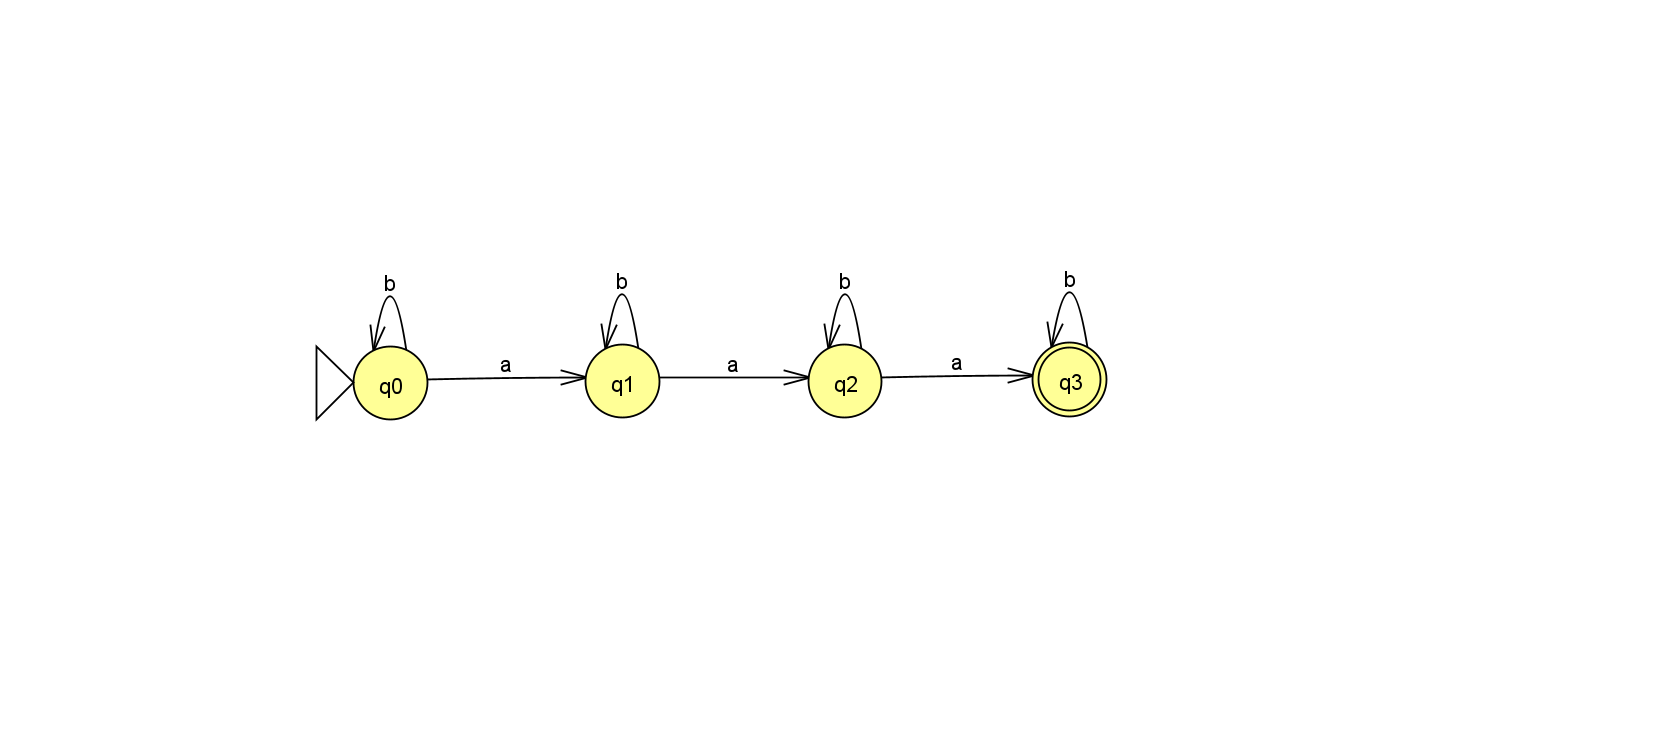
\includegraphics[width=8cm]{pic/1_a1.png}
        \caption{$A_1$的DFA}
        \label{fig1_a1}
        \end{figure}

\begin{figure}
        \centering
        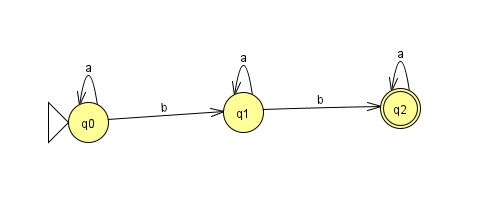
\includegraphics[width=8cm]{pic/1_a2.png}
        \caption{$A_2$的DFA}
        \label{fig1_a2}
        \end{figure}

\begin{figure}
        \centering
        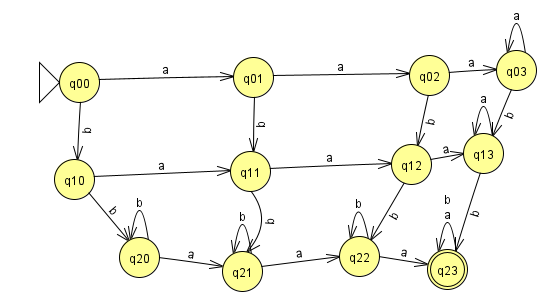
\includegraphics[width=8cm]{pic/1_a3.png}
        \caption{$A_3$的DFA}
        \label{fig1_a3}
        \end{figure}
        
	\part 1.4题(c):$\left\{\omega|\omega\text{偶数个}a\text{和1个或2个}b\right\}$
	\begin{solution}
		令语言$A_1$, $A_2$, $A$, 分别为:
        
        $A_1 = \{x|x\text{含有偶数个a}\}$
        
        $A_2 = \{x|x\text{含有1个或2个b}\}$
        
        $A = A_1 \cup A_2$
        
        则A为题目要求语言。
        
        $A_1$的DFA为图~\ref{fig1_b1}

        $A_2$的DFA为图~\ref{fig1_b2}

        构造$A = A_1 \cup A_2$的DFA为图~\ref{fig1_b3}
        
	\end{solution}

\begin{figure}
        \centering
        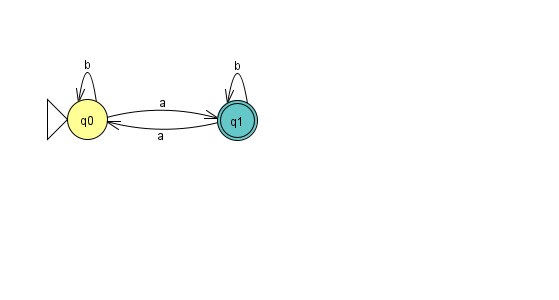
\includegraphics[width=8cm]{pic/1_b1.png}
        \caption{$A_1$的DFA}
        \label{fig1_b1}
        \end{figure}

\begin{figure}
        \centering
        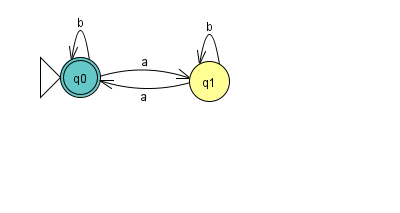
\includegraphics[width=8cm]{pic/1_b2.png}
        \caption{$A_2$的DFA}
        \label{fig1_b2}
        \end{figure}

\begin{figure}
        \centering
        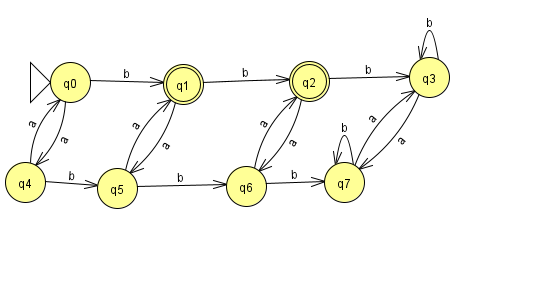
\includegraphics[width=8cm]{pic/1_b3.png}
        \caption{$A_3$的DFA}
        \label{fig1_b3}
        \end{figure}
        
	\part 1.4题(e):$\left\{\omega|\omega\text{从}a\text{开始并且最多1个}b\right\}$
	\begin{solution}
		令语言$A_1$, $A_2$, $A$, 分别为:
        
        $A_1 = \{x|x\text{从a开始}\}$
        
        $A_2 = \{x|x\text{至多1个b}\}$
        
        $A = A_1 \cup A_2$
        
        则A为题目要求语言。
        
        $A_1$的DFA为图~\ref{fig1_c1}

        $A_2$的DFA为图~\ref{fig1_c2}

        构造$A = A_1 \cup A_2$的DFA图~\ref{fig1_c3}
	\end{solution}


\begin{figure}
        \centering
        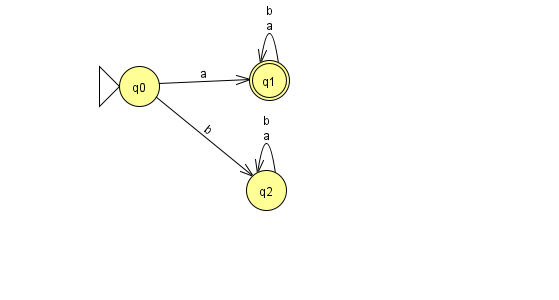
\includegraphics[width=8cm]{pic/1_c1.png}
        \caption{$A_1$的DFA}
        \label{fig1_c1}
        \end{figure}

\begin{figure}
        \centering
        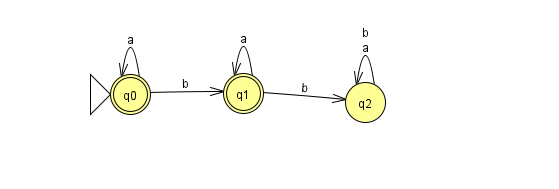
\includegraphics[width=8cm]{pic/1_c2.png}
        \caption{$A_2$的DFA}
        \label{fig1_c2}
        \end{figure}

\begin{figure}
        \centering
        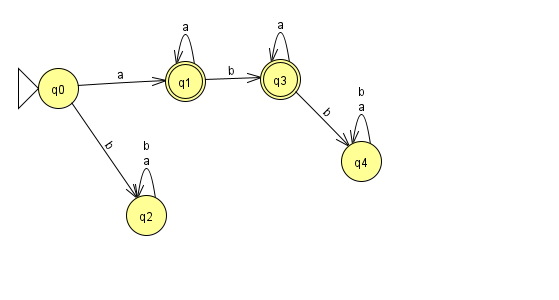
\includegraphics[width=8cm]{pic/1_c3.png}
        \caption{$A_3$的DFA}
        \label{fig1_c3}
        \end{figure}

        
	\part 1.4题(f):$\left\{\omega|\omega\text{含有奇数个}a\text{并且以}b\text{结束}\right\}$
	\begin{solution}
		令语言$A_1$, $A_2$, $A$, 分别为:
        
        $A_1 = \{x|x\text{含有奇数个a}\}$
        
        $A_2 = \{x|x\text{以b结束}\}$
        
        $A = A_1 \cup A_2$
        
        则A为题目要求语言。
        
        $A_1$的DFA为图~\ref{fig1_d1}

        $A_2$的DFA为图~\ref{fig1_d2}

        构造$A = A_1 \cup A_2$的DFA图~\ref{fig1_d3}
	\end{solution}


\begin{figure}
        \centering
        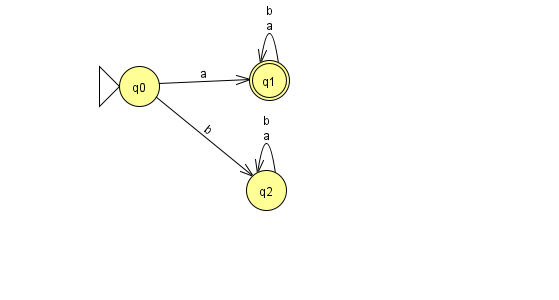
\includegraphics[width=8cm]{pic/1_c1.png}
        \caption{$A_1$的DFA}
        \label{fig1_d1}
        \end{figure}

\begin{figure}
        \centering
        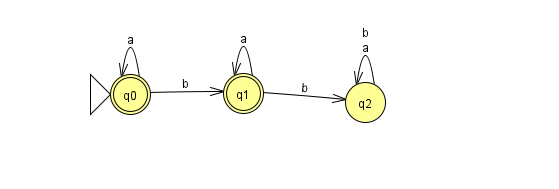
\includegraphics[width=8cm]{pic/1_c2.png}
        \caption{$A_2$的DFA}
        \label{fig1_d2}
        \end{figure}

\begin{figure}
        \centering
        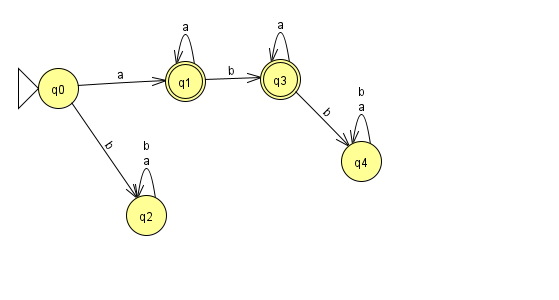
\includegraphics[width=8cm]{pic/1_c3.png}
        \caption{$A_3$的DFA}
        \label{fig1_d3}
        \end{figure}

    
	\part 1.4题(g):$\left\{\omega|\omega\text{的长度为偶数并且有奇数个}a\right\}$
	\begin{solution}
		令语言$A_1$, $A_2$, $A$, 分别为:
        
        $A_1 = \{x|x\text{长度为偶数}\}$
        
        $A_2 = \{x|x\text{有奇数个a}\}$
        
        $A = A_1 \cup A_2$
        
        则A为题目要求语言。
        
        $A_1$的DFA为图~\ref{fig1_e1}

        $A_2$的DFA为图~\ref{fig1_e2}

        构造$A = A_1 \cup A_2$的DFA图~\ref{fig1_e3}
	\end{solution}
\end{parts} 


\begin{figure}
        \centering
        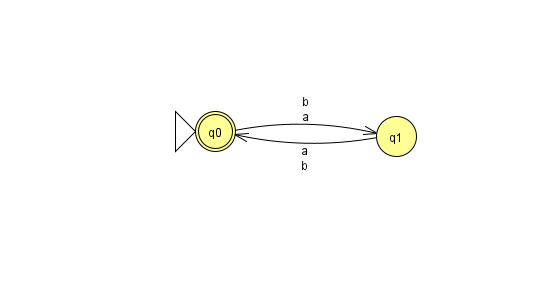
\includegraphics[width=8cm]{pic/1_e1.png}
        \caption{$A_1$的DFA}
        \label{fig1_e1}
        \end{figure}

\begin{figure}
        \centering
        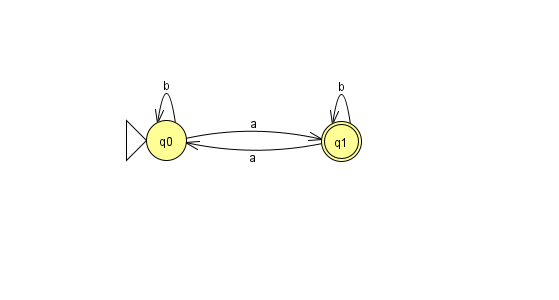
\includegraphics[width=8cm]{pic/1_e2.png}
        \caption{$A_2$的DFA}
        \label{fig1_e2}
        \end{figure}

\begin{figure}
        \centering
        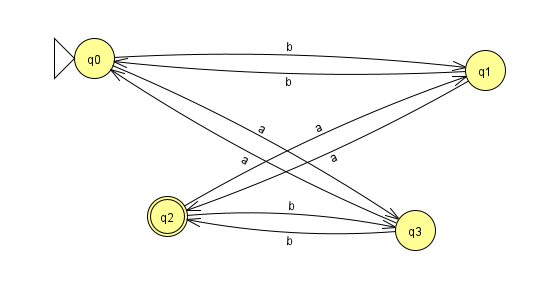
\includegraphics[width=8cm]{pic/1_e3.png}
        \caption{$A_3$的DFA}
        \label{fig1_e3}
        \end{figure}



  \question P51页, 1.5题。
  下述每个语言都是一个简单语言的补。对每一小题先构造简单语言的DFA，然后用其画出给定语言的DFA状态图。在所有问题中$\Sigma=\left\{a,b\right\}$。
  \begin{parts}
	\part 1.5题(c):$\left\{\omega|\omega\text{既不包含子串}ab\text{也不包含子串}ba\right\}$
	\begin{solution}
	    令语言$A_1$, $A$, 分别为:
        
        $A_1 = \{x|x\text{包含子串ab或者包含子串ba}\}$
        
        $A = \complement A_1$
        
        则A为题目要求语言。
        
        $A_1$的DFA为图~\ref{fig2_a1}

        构造$A = \complement A_1$的DFA图~\ref{fig2_a2}
	\end{solution}

\begin{figure}
        \centering
        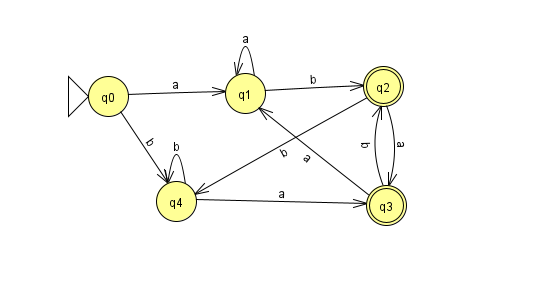
\includegraphics[width=8cm]{pic/2_a1.png}
        \caption{$A_1$的DFA}
        \label{fig2_a1}
        \end{figure}

\begin{figure}
        \centering
        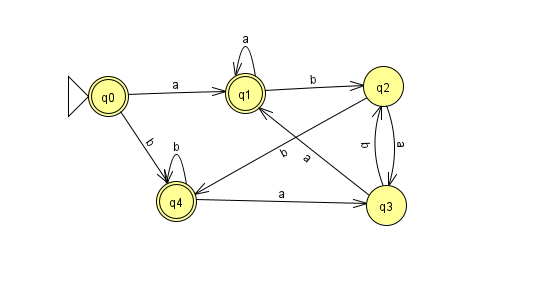
\includegraphics[width=8cm]{pic/2_a2.png}
        \caption{$A_2$的DFA}
        \label{fig2_a2}
        \end{figure}
    
     \part 1.5题(g):$\left\{\omega|\omega\text{是恰好不含2个}a	\text{的任意串}\right\}$
  	\begin{solution}
  	    令语言$A_1$, $A$, 分别为:
        
        $A_1 = \{x|x\text{包含两个a}\}$
        
        $A = \complement A_1$
        
        则A为题目要求语言。
        
        $A_1$的DFA为图~\ref{fig2_b1}

        构造$A = \complement A_1$的DFA图~\ref{fig2_b2}
  	\end{solution}

\begin{figure}
        \centering
        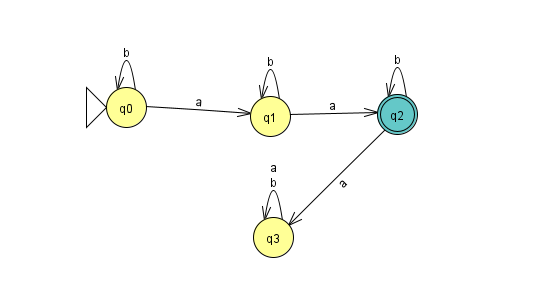
\includegraphics[width=8cm]{pic/2_b1.png}
        \caption{$A_1$的DFA}
        \label{fig2_a1}
        \end{figure}

\begin{figure}
        \centering
        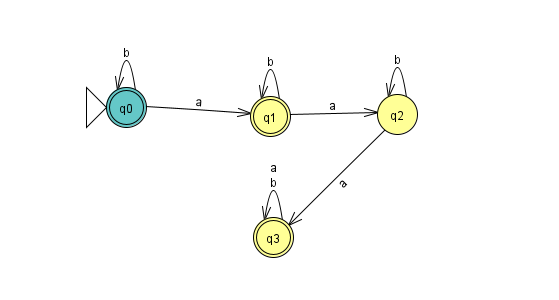
\includegraphics[width=8cm]{pic/2_b2.png}
        \caption{$A_2$的DFA}
        \label{fig2_a2}
        \end{figure}


    
     \part 1.5题(h):$\left\{\omega|\omega\text{是除}a\text{和}b\text{外的任意串}\right\}$
  	\begin{solution}
  	    令语言$A_1$, $A$, 分别为:
        
        $A_1 = \{x|x\text{是a或者b}\}$
        
        $A = \complement A_1$
        
        则A为题目要求语言。
        
        $A_1$的DFA为图~\ref{fig2_c1}

        构造$A = \complement A_1$的DFA图~\ref{fig2_c2}
  	\end{solution}
  \end{parts} 

\begin{figure}
        \centering
        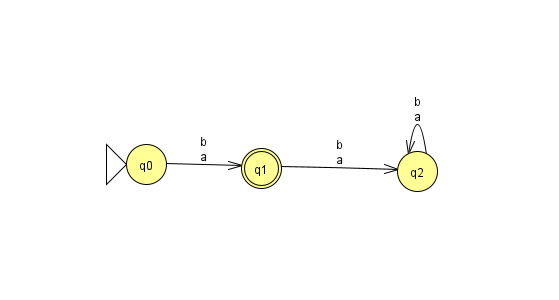
\includegraphics[width=8cm]{pic/2_c1.png}
        \caption{$A_1$的DFA}
        \label{fig2_c1}
        \end{figure}

\begin{figure}
        \centering
        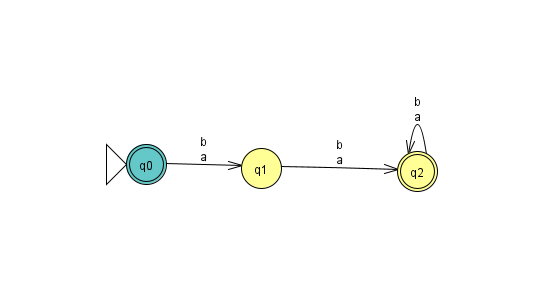
\includegraphics[width=8cm]{pic/2_c2.png}
        \caption{$A_2$的DFA}
        \label{fig2_c2}
        \end{figure}












 
  \question P51页, 1.6题。画出识别下属语言的DFA状态图。在所有问题中字母表均为 $\left\{0,1\right\}$。
  \begin{parts}
	\part 1.6题(e):$\left\{\omega|\omega\text{从0开始且长度为奇数，或从1开始长度为偶数}\right\}$
	\begin{solution}
	       图~\ref{fig3_a}
	\end{solution}
	
	\part 1.6题(h):$\left\{\omega|\omega\text{是除11和111外的任何串}\right\}$
	\begin{solution}
					图~\ref{fig3_b}
	\end{solution}
	
  	\part 1.6题(j):$\left\{\omega|\omega\text{含有至少2个0，并且至多含有1个1}\right\}$
	\begin{solution}
		图~\ref{fig3_c}
	\end{solution} 

	\part 1.6题(l):$\left\{\omega|\omega\text{有偶数个0或恰好2个1}\right\}$
	\begin{solution}
					图~\ref{fig3_d}
	\end{solution}

 \end{parts}

  \begin{figure}
        \centering
        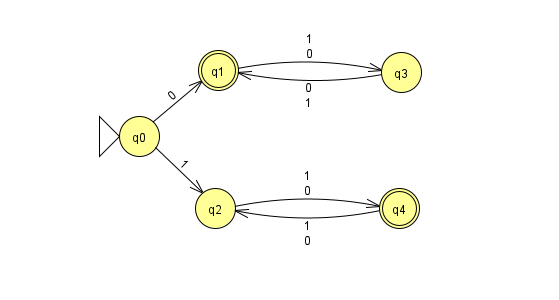
\includegraphics[width=8cm]{pic/3_a.png}
        \caption{3(a)的DFA}
        \label{fig3_a}
        \end{figure}
  \begin{figure}
        \centering
        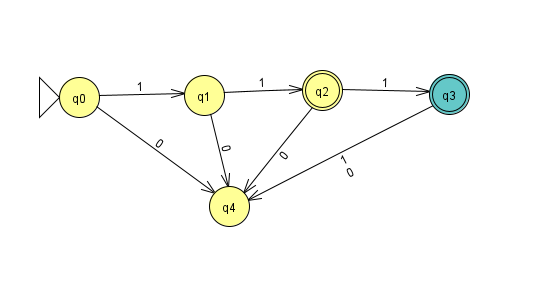
\includegraphics[width=8cm]{pic/3_b.png}
        \caption{3(b)的DFA}
        \label{fig3_b}
        \end{figure}
      \begin{figure}
        \centering
        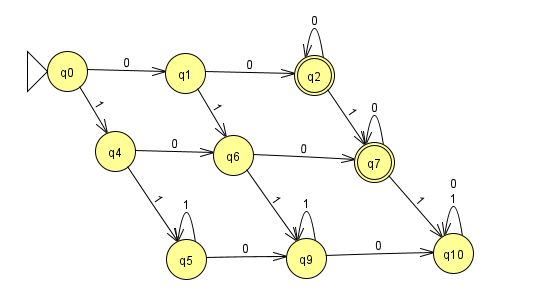
\includegraphics[width=8cm]{pic/3_c.png}
        \caption{3(c)的DFA}
        \label{fig3_c}
        \end{figure}
  \begin{figure}
        \centering
        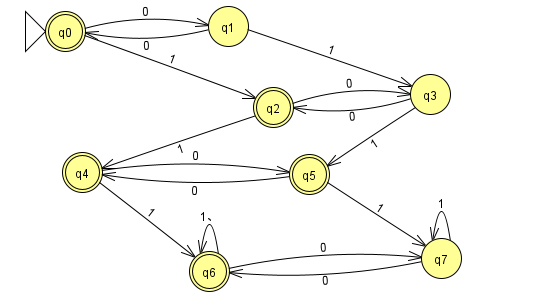
\includegraphics[width=8cm]{pic/3_d.png}
        \caption{3(d)的DFA}
        \label{fig3_d}
        \end{figure}

  \question P52页, 1.14题。
  \begin{parts}
  	\part 证明：若M是一台识别语言B的DFA，交换M的接受状态与非接受状态得到一台新的DFA，则这台新DFA识别B的补集。因而，正则语言类在补运算下封闭。
	\begin{solution}
		设$M_1 = (Q, \Sigma, \delta_1, q_0, F)$是一台识别语言B的DFA。
        
        设集合F在Q上的补为$\complement F$,则DFA:$(Q, \Sigma, \delta_2, q_0, \complement F)$是交换$M_1$接收状态和非接收状态的新DFA.
        
        即，要证明$M_2$识别$\complement B = \Sigma^* - B$

        任取 \( w \in \complement B \)，令 \( w = w_1w_2 \cdots w_n, w_i \in \Sigma \)。将上述的 \( w = w_1w_2 \cdots w_n \) 应用于 DFA \( M_2 \) 中，即用下列方法构造出一个状态序列 \( r_0r_1 \cdots r_n, r_i \in Q \):

        \begin{enumerate}
            \item 令 \( r_0 = q_0 \)，
            \item 对于每个 \( i = 0, 1, \cdots, n-1 \)，令 \( r_{i+1} = \delta_2(r_i, w_{i+1}) \)。
        \end{enumerate}
        
        由于 \( w \notin B \)，而 \( M_1 \) 识别 \( B \)，因此 \( M_1 \) 不接受 \( w \)。
        
        假设 \( r_n \in F \)，由于 \( \delta_1 = \delta_2 \)，则状态序列 \( r_0r_1 \cdots r_n \) 同时满足 \( r_0 = q_0, q_n \in F \)，以及 \( \delta_1(r_i, w_{i+1}) = r_{i+1}, i = 0, 1, \cdots, n \)，则 \( M_1 \) 接受 \( w \)，矛盾。
        
        因此，\( r_n \notin F \)，则 \( r_n \in F \)。因此，状态序列 \( r_0r_1 \cdots r_n \) 同时满足 \( r_0 = q_0, q_n \in F \)，以及 \( \delta_2(r_i, w_{i+1}) = r_{i+1}, i = 0, 1, \cdots, n \)，则 \( M_2 \) 接受 \( w \)。
        
        上面已经证明，对于任取的 \( w \in B \)，都有 \( M_2 \) 接受 \( w \)。因此，\( M_2 \) 识别 \( B \)。因此，正则语言类在补运算下封闭。
	\end{solution} 
  \end{parts}
  
  \question P52页, 1.15题。
  	给出一个反例，说明下述构造不能证明定理1.24，即正则语言类在星号运算下封闭。设$N_{1}=(Q_{1},\Sigma,\delta_{1},q_{1},F_{1})$识别$A_{1}$。如下构造$N=(Q_{1},\Sigma,\delta,q_{1},F)$。$N$应该识别$A_{1}^{*}$\\	
  	a. $N$的状态集是$N_1$的状态集。\\
  	b. $N$的起始状态与$N_1$的起始状态相同。\\
  	c. $F=\{ q_1\}\cup F_1$。$F$的接受状态是原来的接受状态加上它的起始状态。\\
  	d. 定义$\delta$如下：对每一个$q\in Q$和每一个$a\in \Sigma_\varepsilon$，
  	    \begin{equation*}
  	        \delta(q,a)=
  	        \begin{cases}
  	        \delta_1(q,a)&q\not\in F_1 \text{或}a\neq \varepsilon\\ 
  	        \delta_1(q,a)\cup\{q_1\}&q\in F_1 \text{且}a=\varepsilon
  	        \end{cases}
  	    \end{equation*}
  	
  	\begin{solution}
	    下面给出一个 NFA \(N_1 = (\{q_1, q_2, q_3\}, \{0\}, \delta_1, q_1, \{q_3\})\)，其中
        \[
        \delta_1(q, a) =
        \begin{cases} 
        \{q_1\}, & \text{for } q = q_2 \\
        \{q_2\}, & \text{for } q = q_1 \\
        \varnothing, & \text{otherwise}
        \end{cases}
        \tag{6.1}
        \]
        如图~\ref{fig5_1}
        
        根据题中的构造方法，相应地构造出 NFA \(N\)：图~\ref{fig5_2}

        \(N_1\) 识别的语言是 \(\varnothing\)，即 \(A_1 = \varnothing\)，则 \(A_1^* = \{\varepsilon\}\)。而 \(N\) 接收 00，但 00 \(\notin A_1^*\)。

        
	\end{solution}
	      \begin{figure}[htbp]
        \centering
        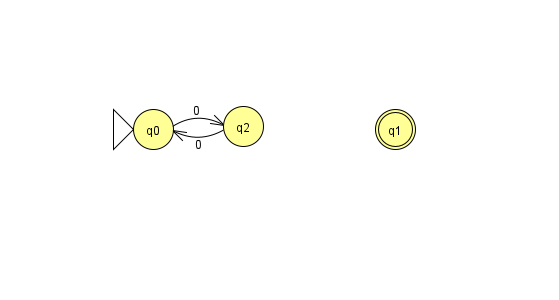
\includegraphics[width=8cm]{pic/5_1.png}
        \caption{题5 DFA1}
        \label{fig5_1}
        \end{figure}
  \begin{figure}[htbp]
        \centering
        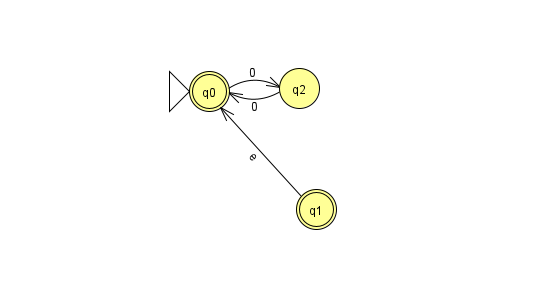
\includegraphics[width=8cm]{pic/5_2.png}
        \caption{题5 DFA2}
        \label{fig5_2}
        \end{figure}
	
    \question P52页, 1.16题, 
    使用定理 1.19 给出的构造，把下图的两台非确定型有穷自动机转换成等价的确定型有穷自动机。
        \begin{figure}[htbp]
	    \centering
	    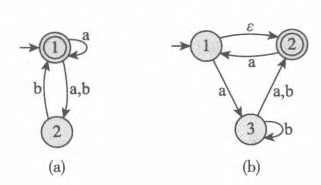
\includegraphics[width=8cm]{1.16.png}
	    \caption{1.16}
	    \label{fig3}
    \end{figure}
    \begin{solution}
	如图~\ref{fig6}
    \end{solution}   
    \begin{figure}[htbp]
        \centering
        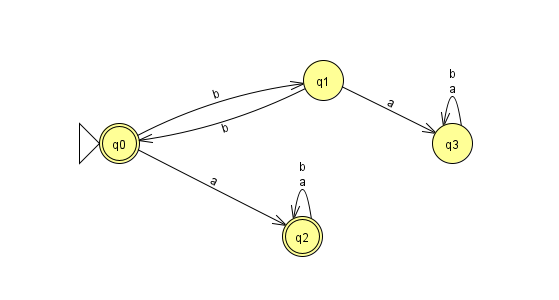
\includegraphics[width=8cm]{pic/6.png}
        \caption{题6 DFA}
        \label{fig6}
        \end{figure}
    \question P52页, 1.19题(b)，使用引理1.29中描述的过程，把下述表达式转换成非确定型有穷自动机。
    $(((00)^*(11))\cup01)^*$ 
	\begin{solution}
		如图~\ref{fig7},其中e代表$\epsilon$
	\end{solution}


  \begin{figure}[htbp]
        \centering
        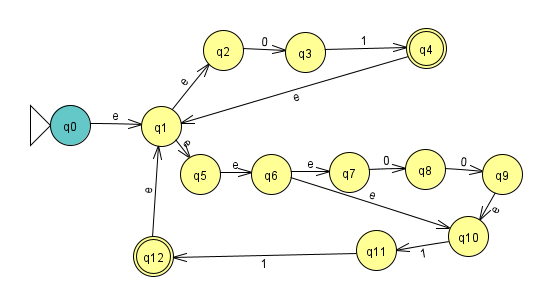
\includegraphics[width=8cm]{pic/7.png}
        \caption{题7 NFA}
        \label{fig7}
        \end{figure}


    
    \question P53页, 1.21题(b), 使用引理1.32中描述的过程，把图中的有穷自动机转换成正则表达式。	
    \begin{figure}[htbp]
	    \centering
	    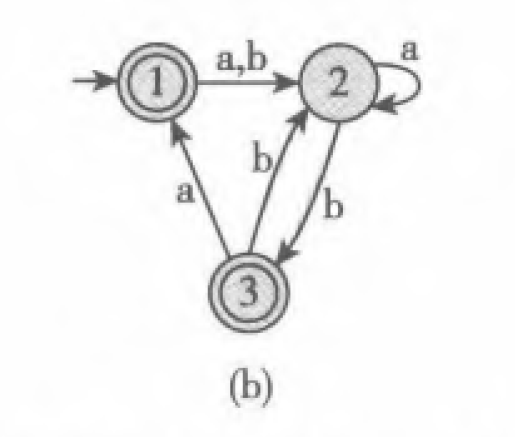
\includegraphics[width=4cm]{1.21(b).png}
	    \caption{1.21(b)}
	    \label{fig4}
    \end{figure}
    \begin{solution}
		$\emptyset \cup ((a \cup b) a^* b) \left((a (a \cup b) \cup b) a^* b\right)^* (\varepsilon \cup a)$
	\end{solution}




    
	\question P53页, 1.22题, 在某些程序设计语言中，注释出现在两个分隔符之间，如$/\#$和$\#/$。设C是所有有效注释串的语言。C中的成员必须以$/\#$开始、$\#/$结束，并且在开始和结束之间没有$\#/$。为了简便起见，假设C的字母表$\Sigma=\left\{a,b,/,\#\right\}$。
  	\begin{parts}
  	\part 给出识别C的DFA。
  	\begin{solution}
		如图~\ref{fig9}
	\end{solution} 

  \begin{figure}[htbp]
        \centering
        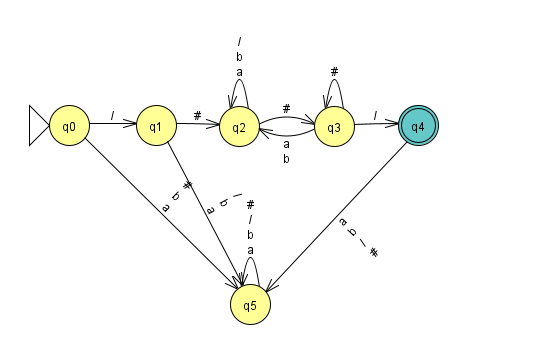
\includegraphics[width=8cm]{pic/9.png}
        \caption{题9 DFA}
        \label{fig9}
        \end{figure}

    
	\part 给出生成C的正则表达式。
	\begin{solution}
		 $/\#(a∪b∪/)∗\#(((a∪b)(a∪b∪/))∗\#)∗/$
	\end{solution} 
	\end{parts}
	\question P53页, 1.28题 (c), 使用定理1.28给出的过程将正则表达式$(a\cup b^+)a^+b^+$转换为NFA, 其中$\Sigma=\{a,b\}$。
	\begin{solution}
		如图~\ref{fig10},其中e代表$\epsilon$
	\end{solution}


  \begin{figure}[htbp]
        \centering
        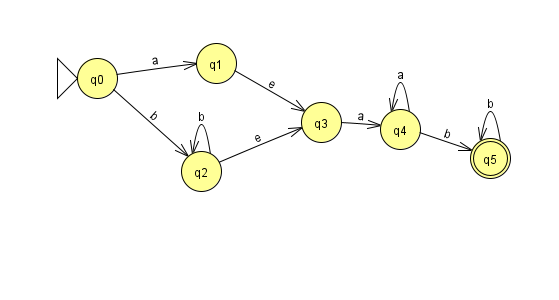
\includegraphics[width=8cm]{pic/10.png}
        \caption{题10 NFA}
        \label{fig10}
        \end{figure}






    
	\question P53页, 1.29题。
使用泵引理证明下述语言不是正则的。


	\begin{parts}
	\part 1.29题(a):$A_1=\left\{0^n1^n2^n|n\geq 0\right\} $
	\begin{solution}
		假设该语言是正则语言，则满足泵引理。设泵长度为 \( p \)。

取该语言内的字符串 \( s = 0^{p+1}2^p \)，长度大于 \( p \)，则可以取 \( s = xyz \)，其中 \( |xy| \leq p \)，又由于 \( |y| > 0 \)，因此字符串 \( y \) 全部由 0 组成。

因此，\( xy^2z \) 也是该语言的字符串，而该字符串中 0 的数量大于 2 的数量，因此该字符串不是该语言内的字符串，矛盾。因此，该语言不是正则的。
	\end{solution}
	
	\part 1.29题(b):$A_2=\left\{\omega\omega\omega|\omega\in \left\{a,b\right\}^{*}\right\}$
	\begin{solution}
		假设该语言是正则语言，则满足泵引理。设泵长度为 \( p \)。取该语言内的字符串
\[
s = a^pba^pba^pb
\]
其长度大于 \( p \)，则可以取 \( s = xyz \)，其中 \( |xy| \leq p \)，又由于 \( |y| > 0 \)，因此字符串 \( y \) 全部由 \( a \) 组成。

因此，\( xy^2z \) 也是该语言的字符串。而
\[
xy^2z = a^{p+|y|}ba^pba^pb
\]
该字符串最后一个字符是 \( b \)，而该字符串只含有三个 \( b \)，而第一个 \( b \) 前的 \( a \) 的数量和最后一个 \( b \) 后 \( a \) 的数量不同，因此该字符串不是该语言内的字符串，矛盾。因此，该语言不是正则的。
	\end{solution}
	
	\part 1.29题(c):$A_3=\left\{a^{2^n}|n\geq 0\right\}$
	\begin{solution}
		假设该语言是正则语言，则满足泵引理。设泵长度为 \( p \) (\( p \geq 1 \))。对于任意的 \( p \)，有  
\[ 2^p > p \]  

取该语言内的字符串 \( s = a^{2^p} \)，长度为 \( 2^p > p \)，则可以取 \( s = xyz \)，其中 \( |xy| \leq p \)，又由于 \( |y| > 0 \)，因此字符串 \( y \) 全部由 a 组成。

因此，\( xy^2z \) 也是该语言的字符串。该字符串为 \( a^{2^p + |y|} \)。假设该字符串是该语言内的字符串，则存在 \( i \geq p + 1 \)，使得  
\[ 2^p + |y| = 2^i \]  

令 \( j = i - p \)，则 \( j \geq 1 \) 且  
\[ 2^p + |y| = 2^{p+j} \]  

则  
\[ |y| = 2^p(2^j - 1) \geq 2^p > p \]  

而 \( |y| \leq |xy| \leq p \)，两式矛盾。因此该字符串不是该语言内的字符串，矛盾。因此，该语言不是正则的。
	\end{solution}
	\end{parts} 
	\question P54页, 1.35题, 设$A/B=\left\{\omega|\text{对于某}x\in B,\omega x\in A\right\}$。证明如果A是正则的，B是任意语言，那么$A/B$是正则的。
	\begin{solution}
		为了证明该结论，对于正则表达式 \( R \)，先按照下列方法定义其长度，记为 \(|R|\):

\[
|R| = 
\begin{cases} 
1, & R = a, \, a \in \Sigma \\
1, & R = \varepsilon \\
1, & R = \varnothing \\
|R_1| + |R_2| + 3, & R = (R_1 \cup R_2) \\
|R_1| + |R_2| + 3, & R = (R_1 \circ R_2) \\
|R_1| + |R_2| + 3, & R = (R_1)^*
\end{cases}
\tag{11.1}
\]

设有符号表 \(\Sigma\)，设 \(A\) 是一个正则语言，设 \(B \subseteq \Sigma^*\)。下面将证明，\(A/B\) 是正则的。

由于 \(A\) 是正则语言，则有一个正则表达式 \(R\) 描述的语言是 \(A\)。对该正则表达式的长度 \(|R|\) 进行归纳。

\subsection*{基础情况：\(|R| = 1\)}
当 \(R\) 的长度为 1 时，\(R\) 要么是 \(a, a \in \Sigma\)，要么是 \(\varnothing\)，要么是 \(\varepsilon\)：

\begin{enumerate}
\item 若 \(R = a, a \in \Sigma\)，则 \(A = \{a\}\)，则 \(A/B = \{w \mid wx \in \{a\}, \, \text{for some } x \in B\}\)，因此
\[
A/B = 
\begin{cases} 
\{a\}, & \text{if } \varepsilon \in B \\
\{\varepsilon\}, & \text{if } \varepsilon \notin B \text{ and } a \in B \\
\varnothing, & \text{otherwise}
\end{cases}
\tag{11.2}
\]
语言 \(\{a\}, \{\varepsilon\}, \varnothing\) 都是正则语言，则 \(A/B\) 是正则的。

\item 若 \(R = \varnothing\)，则 \(A = \varnothing\)，则 \(A/B = \varnothing\)，则 \(A/B\) 是正则的。

\item 若 \(R = \varepsilon\)，则 \(A = \{\varepsilon\}\)，因此
\[
A/B = 
\begin{cases} 
\{\varepsilon\}, & \text{if } \varepsilon \in B \\
\varnothing, & \text{otherwise}
\end{cases}
\tag{11.3}
\]
因此 \(A/B\) 是正则的。
\end{enumerate}

\subsection*{归纳步骤}
假设当 \(|R| < k (k \geq 2)\) 时，待证结论成立，即若 \(A\) 是正则的则 \(A/B\) 是正则的。当 \(|R| = k\) 时，考虑 \(R\) 的构成：

\begin{enumerate}
\item 若 \(R = a, a \in \Sigma\)，上面已经证明此时 \(A/B\) 是正则的。

\item 若 \(R = \varepsilon\)，上面已经证明此时 \(A/B\) 是正则的。

\item 若 \(R = \varnothing\)，上面已经证明此时 \(A/B\) 是正则的。

\item 若 \(R = R_1 \cup R_2\)，假设 \(R_1\) 和 \(R_2\) 描述的语言分别为 \(A_1, A_2\)，则 \(A = A_1 \cup A_2\)，则
\[
\begin{aligned}
A/B &= \{w \mid wx \in A_1 \cup A_2 \text{ for some } x \in B\} \\
&= \{w \mid wx \in A_1 \text{ for some } x \in B\} \cup \{w \mid wx \in A_2 \text{ for some } x \in B\} \\
&= A_1/B \cup A_2/B
\end{aligned}
\tag{11.4}
\]
由于 \(|R_1| < |R| = k, |R_2| < |R| = k\)，因此根据归纳假设 \(A_1/B\) 和 \(A_2/B\) 都是正则的。由于正则语言在并运算下封闭，则 \(A/B\) 也是正则的。

\item 若 \(R = R_1 \circ R_2\)，假设 \(R_1\) 和 \(R_2\) 描述的语言分别为 \(A_1, A_2\)，则 \(A = A_1 \circ A_2\)。构造以下三个集合：
\[
\begin{aligned}
B_1 &= \{x \in B \mid x = x_1 x_2 \cdots, x_i \in \Sigma, \text{存在 } k \geq 1 \text{ 使 } x_k x_{k+1} \cdots \in A_2\} \\
B'_1 &= \{w = x_1 x_2 \cdots x_{k-1} \mid x \in B, x = x_1 x_2 \cdots, x_i \in \Sigma, \text{存在 } k \geq 1 \text{ 使 } x_k x_{k+1} \cdots \in A_2\} \\
B_2 &= \{x \in B \mid x = x_1 x_2 \cdots, x_i \in \Sigma, \text{不存在 } k \geq 1 \text{ 使 } x_k x_{k+1} \cdots \in A_2\}
\end{aligned}
\tag{11.5}
\]
根据定义可知 \(B = B_1 \cup B_2\) 且 \(B_1 \cap B_2 = \varnothing\)。则
\[
\begin{aligned}
A/B &= \{w \mid wx \in A_1 \circ A_2 \text{ for some } x \in B_1 \cup B_2\} \\
&= \{w \mid wx \in A_1 \circ A_2 \text{ for some } x \in B_1\} \cup \{w \mid wx \in A_1 \circ A_2 \text{ for some } x \in B_2\}
\end{aligned}
\tag{11.6}
\]
由于 \(B_1\) 中的串都存在后缀属于语言 \(A_2\)，与这些后缀互补（共同拼成整个串）的一个或若干个前缀位于语言 \(B'_1\) 中，因此
\[
\{w \mid wx \in A_1 \circ A_2 \text{ for some } x \in B_1\} = A_1/B'_1
\tag{11.7}
\]
由于 \(A_1\) 是正则语言，根据归纳假设可得 \(A_1/B'_1\) 也是正则语言。

另一方面，由于 \(B_2\) 中的串的所有后缀都无法被 \(R_2\) 描述，因此
\[
\begin{aligned}
&\{w \mid wx \in A_1 \circ A_2 \text{ for some } x \in B_2\} \\
&= A_1 \circ \{w \mid wx \in A_2 \text{ for some } x \in B_2\} \\
&= A_1 \circ (A_2/B_2)
\end{aligned}
\tag{11.8}
\]
由于 \(A_2\) 是由 \(R_2\) 描述的正则语言，根据归纳假设可得 \(A_2/B_2\) 也是正则语言。由于正则语言在连接运算下封闭，因此 \(A_1 \circ (A_2/B_2)\) 也是正则语言。

综合上述式可得 \(A/B\) 是两个正则语言的并集：
\[
A/B = (A_1/B'_1) \cup (A_1 \circ (A_2/B_2))
\tag{11.9}
\]
因此，\(A/B\) 也是正则语言。

\item 若 \(R = (R_1)^*\)，假设 \(R_1\) 描述的语言是 \(A_1\)。由于 \(A = A_1^0 \cup A_1^1 \cup A_1^2 \cup \cdots\)，因此
\[
\begin{aligned}
A/B &= \{w \mid wx \in A \text{ for some } x \in B\} \\
&= \{w \mid wx \in A_1^0 \cup A_1^1 \cup \cdots \text{ for some } x \in B\} \\
&= \{w \mid wx \in A_1^0 \text{ for some } x \in B\} \cup \{w \mid wx \in A_1^1 \text{ for some } x \in B\} \cup \cdots \\
&= A_1^0/B \cup A_1^1/B \cup A_1^2/B \cup \cdots
\end{aligned}
\tag{11.10}
\]
根据归纳假设，\(A/B\) 也是正则语言。
\end{enumerate}

因此，当 \(|R| = k\) 时，\(A/B\) 也是正则语言。

综上，若 \(A\) 是正则的，则 \(A/B\) 是正则的。
	\end{solution} 






    
    \question P55页, 1.41题。
    设$B_n=\left\{a^k|k\text{是}n\text{的整数倍}\right\}$。证明：对每一个$n\geq 1$，语言$B_n$是正则的。
	\begin{solution}
		下面对任意的 \( n \) 构造 DFA \( D_n = (Q_n, \{a\}, \delta_n, 0, F_n) \)，其识别的语言是 \( B_n \)。

\[
Q_n = \{0, 1, 2, \cdots, n-1\}
\]
\[
F_n = \{0\}
\]
\[
\delta_n(s, a) = (s + 1) \bmod n, \quad s \in Q_n
\]

因此 \( B_n \) 是正则的。
	\end{solution} 




    
    \question P55页, 1.42题。
    设$C_n=\left\{x|x\text{是一个二进制数，且是}n\text{的整数倍}\right\}$。证明：对每一个$n\geq 1$，语言$C_n$是正则的。
	\begin{solution}
		下面对任意的 \( n \) 构造 DFA \( D_n = (Q_n, \{0,1\}, \delta_n, 0, F_n) \)，其识别的语言是 \( C_n \)。

\[
Q_n = \{0, 1, 2, \cdots, n-1\}
\]
\[
F_n = \{0\}
\]
\[
\delta_n(s, a) = (2s + a) \bmod n, \quad s \in Q_n
\]

因此 \( C_n \) 是正则的。
	\end{solution} 

    \question P56页, 1.51题。
    证明下述语言不是正则的。证明可以使用泵引理和正则语言类在并、交、补运算下封闭的性质。
 	
	\begin{parts}
	   \part 1.51题(a):$\left\{0^n1^m0^n|m,n\geq 0\right\} $
		\begin{solution}
		假设该语言是正则语言，则满足泵引理。设泵长度为 \( p \)。

取该语言内的字符串 \( s = 0^{p}10^p \)，长度大于 \( p \)，则可以取 \( s = xyz \)，其中 \( |xy| \leq p \)，又由于 \( |y| > 0 \)，因此字符串 \( y \) 全部由 0 组成。

因此，\( xy^2z \) 也是该语言的字符串，而该字符串中 1 前面的 0 的数量大于 1 后面的 0 的数量，因此该字符串不是该语言内的字符串，矛盾。因此，该语言不是正则的。
		\end{solution}
		
		  \part 1.51题(b):$\left\{0^m1^n|m\neq n\right\}$
	   \begin{solution}
		设 $A$ 为题中语言，$A$ 不是正则的。

假设 $A$ 是正则的，那么 $\overline{A}$ 也是正则的。但
\[
\overline{A} = \{0^m1^m \mid m > 0\}
\]
显然，$\{0^m1^m \mid m > 0\}$ 不是正则的，矛盾。

因此 $A$ 不是正则的。
		\end{solution}
		
	   \part 1.51题(c):$\left\{\omega|\omega\in \left\{0,1\right\}^{*}\text{不是一个回文}|\right\}$
	   \begin{solution}
		设
\[
A = \{ w \mid w \in \{0,1\}^* \text{ 不是一个回文} \}
\]
\[
B = \{ w \mid w \in \{0,1\}^* \text{ 是一个回文} \}
\]

先证明 \( B \) 不是正则的。

假设 \( B \) 是正则语言，则满足泵引理，设泵长度为 \( p \)。取该语言内的字符串 \( s = 0^p 10^p \)，长度大于 \( p \)，则可以取 \( s = xyz \)，其中 \( |xy| \leq p \)，又由于 \( |y| > 0 \)，因此字符串 \( y \) 全部由 0 组成。

因此，\( xy^2z \) 也是该语言的字符串，而该字符串中 1 前的 0 的数量大于 1 后 0 的数量且只有一个 1，因此该字符串不是回文，因此也不是 \( B \) 内的字符串，矛盾。因此，\( B \) 不是正则的。

假设 \( A \) 是正则语言，则 \( \overline{A} \) 也是正则语言。而 \( \overline{A} = B \)，\( B \) 不是正则语言，矛盾。因此 \( A \) 不是正则的。
		\end{solution}
		
	 \part 1.51题(d):$\left\{\omega t\omega|\omega,t\in \left\{0,1\right\}^{+}\right\} $
		\begin{solution}
		假设该语言是正则语言，则满足泵引理，设泵长度为 \( p \)。取该语言内的字符串
\[
s = 0^p 110^p 1
\]
其长度大于 \( p \)，则可以取 \( s = xyz \)，其中 \( |xy| \leq p \)，又由于 \( |y| > 0 \)，因此字符串 \( y \) 全部由 0 组成。因此
\[
xy^2z = 0^{p+|y|} 110^p 1
\]
也是该语言的字符串。

假设该字符串是该语言内的字符串。其最后一个字符是 1，而该语言要求字符串的某个相同长度的前后缀相同，因此该字符串需要存在一个以 1 结尾的前缀。第一个 1 出现在第 \( p + |y| \) 位，前面都为 0，而该字符串尾部除了 1 外，最多只有 \( p \) 个 0。因此，该字符串不是该语言内的字符串，矛盾。因此，该语言不是正则的。
		\end{solution}	
		
		
	\end{parts} 
	\question P56页, 1.52题。
    设$\Sigma=\left\{1,\# \right\}$以及$Y=\left\{\omega|\text{对}k\geq 0,x_i\in 1^*\text{且}i\neq j\text{时} x_i\neq x_j,\omega=x_1\#x_2\#...\#x_k\right\}$,证明：$Y$不是正则的。
	\begin{solution}
		假设该语言是正则语言，则满足泵引理，设泵长度为 \( p \)。取该语言内的字符串
\[
s = 1^p \# 1^{p-1} \# \cdots \# 1 \#
\]
其长度大于 \( p \)，则可以取 \( s = xyz \)，其中 \( |xy| \leq p \)，又由于 \( |y| > 0 \)，因此字符串 \( y \) 全部由 1 组成。

因此，删除 \( y \) 后得到的字符串
\[
xz = 1^{p-|y|} \# 1^{p-1} \# 1^{p-2} \# \cdots \# 1 \#
\]
也是该语言的字符串。

其中 \( 1 \leq |y| \leq p \)，因此 \( p - |y| \) 至少和一个从 \( p - 1 \) 到 0 之内的数相同，因此该字符串不是该语言内的字符串，矛盾。因此该语言不是正则的。
	\end{solution} 



    
	\question P57页, 1.68题。设$\Sigma=\left\{0,1\right\}$,
    \begin{parts}
  	    \part 若$A=\left\{0^k u 0^k|k\geq 1\text{并且} u\in \Sigma^*\right\}$
  	    证明：$A$是正则的。
        \begin{solution}
		$A=\{0u0|u\in \Sigma∗\}$，因此可以用图~\ref{fig17}的NFA判定
	    \end{solution} 
	      \begin{figure}[htbp]
        \centering
        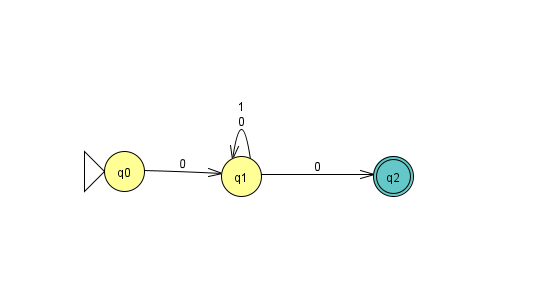
\includegraphics[width=8cm]{pic/17.png}
        \caption{题17 NFA}
        \label{fig17}
        \end{figure}
	    \part 若$B=\left\{0^k1u0^k|k\geq 1\text{并且} u\in \Sigma^*\right\}$
  	    证明：$B$不是正则的。
        \begin{solution}
		假设 \( B \) 是正则的，令 \( p \) 为泵引理给出的泵长度，选择 \( s \) 为 \( 0^{p}10^p \)。  
泵引理保证 \( s \) 可以被划分为三片，即 \( s = uvw \)，且 \( |uv| \leq p \)。因此，\( v \) 中仅含有 0，设 \( v = 0^m \)。根据泵引理，应当有字符串 \( uv^2w = 0^{p+m}10^p \in B \)。  
根据 \( B \) 定义，此时 \( k = p + m > p \)，结尾没有连续的 \( k \) 个 0。因此 \( uv^2w \notin B \)，矛盾！  
因此 \( B \) 不是正则的。
	    \end{solution} 
	    
    \end{parts}
    \question P57页, 1.71题。
    \begin{parts}
  	    \part 设$B=\left\{1^ky| y\in \left\{0,1\right\}^{*},\text{并且对} k\geq 1,y\text{含有至少}k\text{个}1\right\}$
  	    证明：$B$是正则语言。
	    \begin{solution}
		$B=\{1y|y\in \{0,1\}∗,y含有至少1个1\}$，可以用图~\ref{fig18}的DFA判定
	    \end{solution} 
\begin{figure}[htbp]
        \centering
        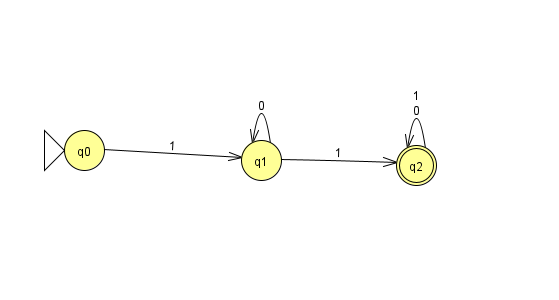
\includegraphics[width=8cm]{pic/18.png}
        \caption{题18 NFA}
        \label{fig18}
        \end{figure}
        
	    \part 设$C=\left\{1^ky| y\in \left\{0,1\right\}^{*},\text{并且对} k\geq 1,y\text{含有至多}k\text{个}1\right\}$
  	    证明：$C$不是正则语言。
        \begin{solution}
		假设 \( C \) 是正则的，令 \( p \) 为泵引理给出的泵长度，选择 \( s \) 为 \( 1^p01^p \)。

泵引理保证 \( s \) 可以被划分为三片，即 \( s = uvw \)，且 \( |uv| \leq p \)。因此，\( v \) 中仅含有 1，设 \( v = 1^m \)。根据泵引理，应当有字符串 \( uv^0w = 1^{p-m}01^p \in C \)。

根据 \( C \) 定义，此时 \( k \leq p - m \)，\( y = 1^{p-m-k}01^p \)，含有至少 \( p > k \) 个 1。因此 \( uv^0w \notin C \)，矛盾！因此 \( C \) 不是正则的。
	    \end{solution} 
  \end{parts}

\end{questions}

\end{document}

%%% Local Variables: 
%%% mode: latex
%%% TeX-master: t
%%% End: 
